Before
we discuss previous works on question answering (QA),
we first look at the settings that QA systems
are designed to operate on.
% Aligning with the motivation in Chapter~\ref{chp:intro},
% we focus on two aspects of such settings.
First, Section~\ref{sec:rw-knowledge-sources}
analyzes the types of \emph{knowledge sources} that QA
systems pull information from.
We describe and contrast the nature of
structured, unstructured, and semi-structured data,
with a special emphasis on the sorts of information they tend to contain
and the challenges they pose to the QA systems.
Then in Section~\ref{sec:rw-questions},
we look at the \emph{types of questions} different QA systems
are designed to handle.
We particularly focus on \emph{fact-based}\footnote{While
questions with factual answers
are sometimes called ``factoid'' questions,
the term ``factoid'' sometimes denotes simple questions
that do not need complex reasoning.
We use the term ``fact-based'' to avoid confusion.}
questions and highlight the various types of complexity
that can be present in the questions.

Afterward, we review the two main lines of work on question answering.
First, Section~\ref{sec:rw-retrieval-based-qa}
explores \emph{retrieval-based QA} systems.
As the name suggests,
these QA systems
first retrieve snippets from the knowledge source
that are relevant to the question,
and then use reading comprehension to extract the answer
from the retrieved snippets.
Second, in Section~\ref{sec:rw-knowledge-based-qa},
we look at \emph{knowledge-based QA} systems,
which perform
reasoning on the structure of the knowledge source
to compute the answer.
We particularly focus on the \emph{semantic parsing} approach,
which we use for the main task of this dissertation.

\begin{figure}[t]
\centering
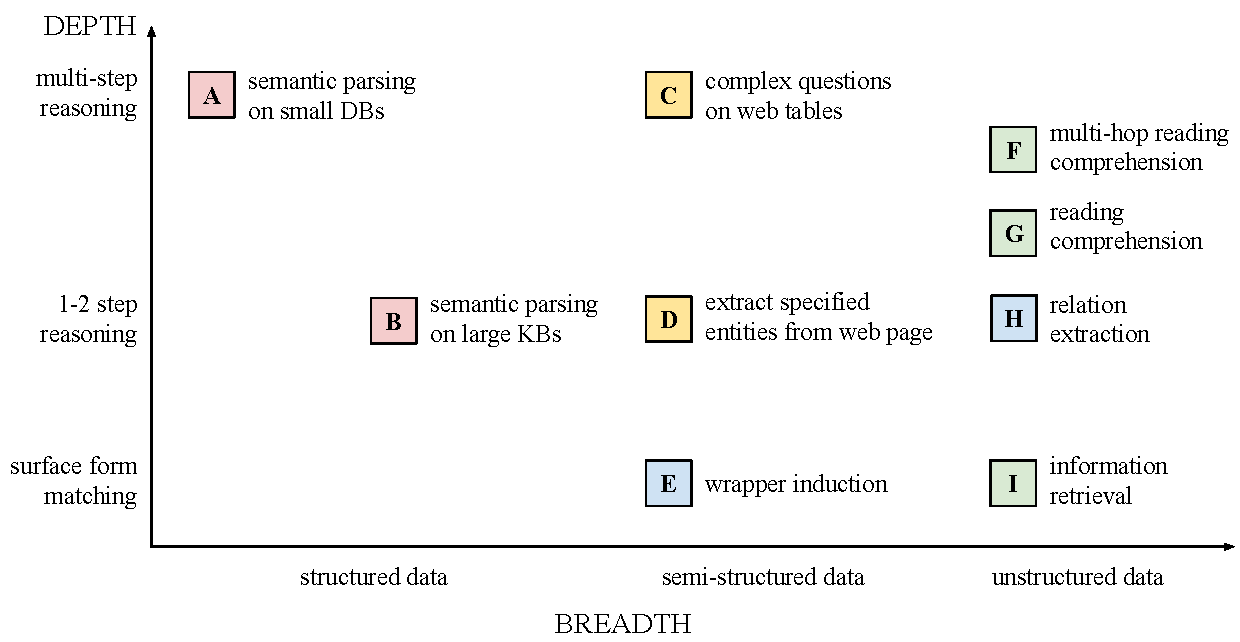
\includegraphics[width=\textwidth]{figures/intro/breadth-depth.pdf}
\caption
[Comparison of related work in terms of \Breadth and \Depth]
{Comparison of retrieval-based QA (green),
knowledge-based QA (red),
and information extraction systems (blue) on
the scope of the knowledge source (\Breadth)
and the question complexity (\Depth).
This dissertation starts
with exploring semi-structured data
(Point~D),
and then progresses to a task that addresses
both \Breadth and \Depth
simultaneously (Point~C).}
\label{fig:depth-breadth-plot}
\end{figure}

These two classes of QA systems
traditionally operate on the opposite ends
of the spectrum.
As illustrated in Figure~\ref{fig:depth-breadth-plot},
retrieval-based QA works on open-domain unstructured data
(high \Breadth)
but traditionally aims to answer questions
that do not require multi-step reasoning
(low \Depth).
In contrast,
the strength of knowledge-based QA is its ability to
perform multi-step reasoning to answer complex questions
(high \Depth),
but the knowledge sources are traditionally constrained
to structured data with predefined schemata,
such as databases or knowledge bases
(low \Breadth).
The goal of this dissertation
(and several other recent works)
is to build QA systems that can
operate in high-\Breadth high-\Depth settings.

Finally in Section~\ref{sec:rw-ie},
we discuss \emph{information extraction} (IE) systems.
An IE system transforms unstructured or semi-structured data
into the structured format that knowledge-based QA systems can process,
which allows them to answer questions that are both complex
and open-domain.
The goal of most IE systems in the literature is to populate
a central structured knowledge source with a predefined schema.
While this allows information from multiple sources to be aggregated
in a systematic manner,
%this pipeline paradigm
%(extract information to get structured data, then apply QA)
the predefined schema,
along with precision and recall issues,
%this paradigm
%has several downsides that
inherently limits the amount of knowledge accessible by
the downstream systems.
As an alternative, the work in this dissertation employs
\emph{on-the-fly information extraction}:
instead of populating a central fixed-schema database,
we only convert parts of the source data
that are relevant to the question
into a temporary structured knowledge source.
Without a predefined schema, we are able to capture
more information from the source data;
however, we lose some benefits of having a unified database
(e.g., we can no longer aggregate data from different sources,
and running extraction for every question can be costly).
% We now also need a better QA system
% that can handle arbitrary data schemata.

%%%%%%%%%%%%%%%%%%%%%%%%%%%%%%%%%%%%%%%%%%%%%%%%%%%%%
\section{Knowledge sources}
\label{sec:rw-knowledge-sources}

We now classify the types of knowledge sources used
in QA systems based on
(1) the amount of structure specified
in the knowledge sources and
(2) whether the data schema is predefined.
The \Breadth axis in
Figure~\ref{fig:depth-breadth-plot}
lays out the different types of knowledge sources
described below.


\subsection{Structured data}

A structured knowledge source
has a well-defined \emph{schema}, which dictates
the types of objects that can exist in the knowledge source,
as well as the types of relations among them.
Database is a canonical example of structured knowledge sources:
the database schema defines the value type in each field,
the fields in each record,
and the relationship between records across database tables.
Other examples of structured knowledge sources
include
%databases (often contain data in some specific domain),
graph-structured
knowledge bases \cite{freebase2013dump,suchanek2007yago,auer2007dbpedia}
%(large and open-domain,
%with the types of graph nodes and edges defined by designers)
and constrained interactive environments
(e.g., a simulated world
with blocks that can be moved around).
Most knowledge-based QA systems,
such as natural language interfaces to databases \cite{androutsopoulos95nlidb}
and semantic parsers
\cite{zelle96geoquery,berant2013freebase,chen11navigate}
operate on structured knowledge sources.

Using a structured knowledge source
provides several benefits.
A structured knowledge source can store
a large amount of statistical data,
and usually provides a convenient interface
(e.g., database query languages)
for performing computation on such statistics.
Furthermore, structured data is a systematic way to consolidate knowledge.
In contrast to unstructured text
which may describe the same object,
relation, or event using a wide variety of paraphrases,
the schema of structured data forces the representation of information
to be unified and canonicalized,
making it easier to process.

On the flip side,
structured data presents a trade off between
knowledge coverage and maintainability.
Closed-domain structured knowledge sources,
such as a database for a specific application,
only support questions that are asked within that domain.
On the other hand,
open-domain structured knowledge sources,
such as large knowledge bases,
support a wider range of questions but
are difficult to populate and maintain.

Finally,
the fixed schema in structured data is both a blessing and a curse.
It is easier to design or learn a mapping between
natural language phrases in the question
and objects in the knowledge source
when the schema is known in advance.
However, the fixed schema limits the types
of knowledge that can be included in the knowledge source.

\subsection{Unstructured data}
\label{sec:rw-unstructured-data}

Unstructured knowledge sources are knowledge sources that
do not contain a schema.
While some QA works operate on \emph{unstructured media}
 such as 
images or videos,
most retrieval-based QA systems 
operate on \emph{unstructured text},
which we will focus on for our comparison.

A large amount of open-domain world knowledge is encoded
as unstructured text due to the flexibility
and expressiveness of natural language.
Apart from describing objects and their properties,
%as commonly seen in structured knowledge sources,
unstructured text is also used to express more complex structures
such as events and processes,
or more vague concepts such as arguments and opinions.
Using unstructured data as the knowledge source
opens the door for a much wider range of questions.

As its downside, unstructured text is more difficult
to process than structured data.
Due to the flexibility of natural language,
a QA system must be ready to handle
different sentence structures and 
linguistic patterns people use to express the same concept.
Additionally, compared to structured data,
plain text is a more clunky way to express a long series
(e.g., list of all national parks in United States)
or statistical data
(e.g., the area of each national park).
This means unstructured data is less suitable for questions
that require computation;
for instance, the data needed for computing the average area
of national parks is less likely to be expressed in plain text
(except when the average is already computed and explicitly stated in text).

\subsection{Semi-structured data}
\label{sec:rw-semi-structured-data}

Semi-structured data contains some semantic structures,
but the schema of such structures is not predefined
\cite{abiteboul1997querying,mchugh1997lore}.
Examples of semi-structured data include markup documents
(e.g., schema-less XML files and HTML pages)
and sections with uniform patterns within a document
(e.g., tables, bullet lists, and template-generated product listings
on web pages).
While a spcific data source might use the same schema
for all of its documents,
that schema would not apply to the similar type of content
from a different data source.

Semi-structured data inherits the advantages and disadvantages
from both structured and unstructured data.
Similar to structured data,
semi-structured data usually contains computable data,
but since the schema is not predefined,
it can express a variety of open-domain knowledge
depending on the author of the data.
On the flip side, the lack of a predefined schema
increases the difficulty of mapping
phrases in the questions to objects in the knowledge source.

%%%%%%%%%%%%%%%%%%%%%%%%%%%%%%%%%%%%%%%%%%%%%%%%%%%%%
\section{Types of questions}
\label{sec:rw-questions}

We now discuss the types of questions targeted by previous work
in question answering.
The family of questions our work focuses on is \emph{fact-based}
questions,
which have objective and mostly unique answers
with respect to the knowledge source
(e.g., \nl{Where was Barack Obama born?}
or \nl{What is the average earning of the company in 1999?}).
% Some previous works refer to these questions as
% \emph{factoid} questions,
% though the term ``factoid'' also carries the connotation of
% trivia-like questions that do not require complex reasoning to answer.
%
Other than fact-based questions,
previous work has also considered questions
whose answers are long explanations or opinions
\cite{burke1997question,soricut2006automatic}.
Most systems for answering such open-ended questions
treat the task as a information retrieval task,
where the potential answer snippets are retrieved and then ranked.

\subsection{Complexity in fact-based questions}

Most retrieval-based and some knowledge-based QA systems
target fact-based questions that only require simple reasoning
(sometimes called ``factoid'' questions).
As an example, consider the question
\nl{Where was Barack Obama born?}
asked under different knowledge sources.
When the knowledge source is a corpus of text documents,
a retrieval-based QA system can fetch a snippet that is likely
to contain the answer
(e.g., \nl{Obama was born on August 4 \dots in \textbf{Honolulu, Hawaii}.} from
the Wikipedia article \emph{Barack Obama}),
and then extract the answer
\nl{Honolulu, Hawaii} directly from a sentence in that snippet.
On the other hand, if the knowledge source is a structured database,
a knowledge-based QA system can identify the relevant entity
(\emph{Barack Hussein Obama})
and relation
(\emph{place of birth})
to find the answer.
In either cases,
given a portion of the knowledge source relevant to the question,
the answer can be computed using few steps of reasoning.

As stated in Chapter~\ref{chp:intro},
we want to build QA systems
that can answer complex questions
(i.e.,
high on the \Depth axis in Figure~\ref{fig:depth-breadth-plot}).
% but this does not necessarily means the questions
% have to be long or unnatural.
We consider the following sources of complexity
that can arise in fact-based questions.

\paragraph{Multi-step reasoning.}
% Many questions cannot be answered just by a single step of reasoning.
Performing multiple steps of reasoning
has been the goal of many knowledge-based QA
and interactive systems.
As an example, consider an early conversational system SHRDLU
\cite{winograd1972language},
which takes natural language commands or questions,
manipulates blocks in a simulated
three-dimensional environment,
and then generates natural language responses.
SHRDLU was designed to understand complex commands such as
\nl{Find a block which is taller than the one you are holding
and put it into the box.}
and
\nl{Is at least one of them narrower than the one which
I told you to pick up?}
(where \emph{them} refers to the answer from the previous question).
Another example is an early semantic parsing system
by \citet{zelle96geoquery},
which aims to answer highly compositional questions
such as
\nl{What states border states that border states that border states that border Texas?}
using a database as the knowledge source.

One common criticism of targeting multi-step reasoning
is the argument that humans rarely ask questions with complex linguistic constructs.
Indeed, since most commercial retrieval and question answering systems
(e.g., search engines and early virtual assistants)
cannot understand complex questions well,
the users have learned to ask simple questions
or even use a fragmented list of words
for such products.
Nevertheless, with the introduction of speech-enabled devices,
users have started to use natural language more often,
which increases the frequency of questions
that require multiple steps of reasoning
(though not as many steps as the examples given above).
% \citex.

\paragraph{Sublexical compositionality.}
Multi-step reasoning does not necessarily come from
questions with high linguistic compositionality.
Rather, depending on the type of information available in
the knowledge source,
even a simple word or phrase and invoke multi-step reasoning.
An example of such \emph{sublexical compositionality}
\cite{wang2015overnight}
is the question
\nl{Who is Barack Obama's \textbf{aunt}?}.
The question only requires one step of reasoning
if the knowledge source explicitly mentions the \emph{aunt} relationship.
However, for a database where only a person's parents,
siblings, and gender can be queried,
multiple steps of reasoning will be needed to answer the question.
Several other examples include
\nl{weekend} (Saturday or Sunday),
\nl{same position as John}
(people with the same position as John, except John himself),
and \nl{win} (might require summing up the scores to be compared).

\paragraph{Diversity of operators.}
Another potential source of complexity in fact-based questions
comes from the types of reasoning needed to compute the answer.
For instance, a QA system dealing with statistics
should be able to perform comparison
(\nl{Which company has the highest revenue?}),
aggregation
(\nl{What is the average revenue of tech companies?}),
and computation
(\nl{How much more does Walmart make than Apple?})
on the numerical data in the knowledge source.

As we will discuss in Section~\ref{sec:rw-knowledge-based-qa},
many knowledge-based QA systems use \emph{logical operators}
to represent types of reasoning.
Within this framework, the system has to choose the correct
logical operators, their arguments, and the order they should be composed
to compute the answer.
This can be challenging as the number of possible combinations
of operators scales with the size of the knowledge source
and grows exponentially with the number of reasoning steps.

%%%%%%%%%%%%%%%%%%%%%%%%%%%%%%%%%%%%%%%%%%%%%%%%%%%%%
\section{Retrieval-based question answering}
\label{sec:rw-retrieval-based-qa}

We now discuss the first family of question answering systems,
retrieval-based QA,
which is often used to handle open-domain questions
on unstructured knowledge sources.
To answer a given fact-based question,
most retrieval-based QA systems
(1) retrieve snippets from the knowledge source
that are relevant to the question,
and then (2) use reading comprehension to extract the answer
from the retrieved snippets.

\paragraph{Snippet retrieval.}
Given the question,
the task of snippet retrieval is to fetch portions of the knowledge source
that are relevant to the question,
and then rank them based on relevancy.

For fetching the candidate snippets to be ranked,
the most basic method is to find documents
with large word overlap with the question.
Weighting schemes such as tf-idf is often used
to emphasize the matching of important content words
\cite{jones1972tfidf,robertson2009probabilistic}.
To increase recall,
previous work has also used query expansion and query rewriting
to generate similar queries for retrieving a larger number
of relevant snippets
\cite{carpineto2012expansion}.

Various factors can be considered when ranking the snippets.
For instance, given user ratings as training data,
previous work considered training a supervised model
to assign scores to the retrieved snippets
\cite{cao2006adapting,yue2007support}.
Other factors such as prominence or credibility of the sources
can also be taken into account
\cite{haveliwala2002topic,gyongyi2004combating}

\paragraph{Reading comprehension.}
Given a snippet for the question,
the next step is to extract the answer from the snippet.
Early work in reading comprehension analyzes the question type
and uses linguistics patterns to extract the answer
\cite{brill2002askmsr,pasca2003open}.
With the availability of larger datasets and neural models,
more recent works cast reading comprehension as
predicting a token span inside the given snippet
\cite{yang2015wikiqa,rajpurkar2016squad,seo2016bidaf}.
This generally involves embedding the snippet and the question,
computing interaction between the two,
and then outputting the start and end positions of the span.
For fact-based questions with few steps of reasoning,
such neural models have matched the human performance
on many benchmarks \cite{chen2016thorough,devlin2018BERT}.

\paragraph{Increasing question complexity.}
Traditionally,
the questions that retrieval-based QA applies on
are usually ``factoid'' questions
that do not involve multi-step reasoning
\cite{voorhees1999overview,brill2002askmsr,pasca2003open}.
However,
more recent work has started to move toward
questions that require more complex reasoning.
% Early question answering systems
% (Point~J in Figure~\ref{fig:depth-breadth-plot})
% focus on retrieving the documents
% related to the question
% and extracting the relevant passage.
% The task of extracting more fine-grained answers
% started off with answer span extraction
% (Point~H)
% usually involving locating the correct context in a paragraph
% or document
% Later reading comprehension tasks
% demand more complex reasoning
% (Point~G):
% determining if a question is answerable
% requires reasoning beyond surface form matching
% \cite{rajpurkar2018squadrun},
% and many datasets contain
% questions with multi-hop reasoning over multiple pieces of evidence
% \cite{yang2018hotpotqa,dua2019drop}.
For instance,
datasets such as SQuAD 2.0 \cite{rajpurkar2018squadrun}
and Natural Questions \cite{kwiatkowski2019natural}
require the system to reason whether the question can be answered
by the given snippet.
The DROP dataset \cite{dua2019drop}
contain questions that require various types of operations
such as cross-referencing, comparison, and calculation
to compute the answer.
And the HotpotQA dataset \cite{yang2018hotpotqa}
requires two-step reasoning
where a second snippet has to be retrieved
based on the information gained from the first snippet.

Nevertheless, the types of questions and their complexity
are still partially limited by the nature of the knowledge source.
As discussed in Section~\ref{sec:rw-unstructured-data},
questions that require aggregating the attributes
of many entities 
(e.g., \nl{What is the average revenue of \dots?}
or \nl{Who is the oldest \dots?}) are usually covered by structured
or semi-structured data rather than unstructured text.

\paragraph{Question answering on images.}
As a side note,
a similar trend of increased question complexity
has also been observed
in the related task of visual question answering.
After the success of object recognition
\cite{krizhevsky2012imagenet,szegedy2015googlenet,he2016resnet}
and image captioning
\cite{farhadi2010every,lin2014microsoft,fang2015captions,mao2015deep},
researchers turned to the task of answering questions about the images.
Most earlier works consider
either simpler questions on diverse images \cite{antol2015vqa}
or complex questions on synthetic images \cite{johnson2017clevr,suhr2017nlvr}.
However, recent work has moved toward considering
higher \Breadth and \Depth simultaneously:
understanding complex questions
in the context of open-domain images
\cite{suhr2018situated,hudson2019gqa}.

%%%%%%%%%%%%%%%%%%%%%%%%%%%%%%%%%%%%%%%%%%%%%%%%%%%%%
\section{Knowledge-based question answering}
\label{sec:rw-knowledge-based-qa}

Knowledge-based QA systems perform reasoning on the facts
in the knowledge source
to compute the answer.
Among different ways to perform reasoning,
we focus on the \emph{semantic parsing} approach,
which we use for our main task.
In semantic parsing,
the steps of computation are represented as a discrete representation
called a \emph{logical form},
and the task is thus to map the given question into a logical form
that represents a correct way to compute the answer.

\subsection{Executable semantic parsing}

Broadly speaking,
\emph{semantic parsing} is the task of mapping
natural language utterance to \emph{some}
meaning representation.
As different subfields of natural language processing
employ different schemes of meaning representations,
the term ``semantic parsing''
has become a heavily overloaded term.
The possible interpretations include
shallow intent-slot tagging in dialog systems
\cite{pieraccini1991stochastic,raymond2007generative,mesnil2014using},
identifying semantic frames \cite{gildea02semantic,hermann2014semantic},
and
generating full semantic representations
such as abstract meaning representation (AMR) \cite{banarescu2013amr,flanigan2014discriminative,wang2015transition,artzi2015broad}
among many others.

For the purpose of question answering,
we will focus on \emph{executable semantic parsing},
which is based on
model-theoretic formal semantics \cite{montague73ptq}.
In this framework,
the semantic representations are interpreted under
the knowledge source (traditionally called a ``model'').
The result of this interpretation is called \emph{denotation},
which denotes some part of the knowledge source.
For instance,
in a database of countries in the world,
the denotation of $\T{CapitalOf}(\T{France})$
is a single entity $\T{Paris}$,
while the denotation of $\T{CapitalOf}$
is the mapping between countries and their capital cities.

In practical terms,
executable semantic parsing
is the task of mapping the input utterance $x$
into a semantic representation $z$
(usually called \emph{logical forms})
that can be executed like a computer program
on the knowledge source $w$
to give some desired denotation $y = \deno{z}{w}$.
For instance, the utterance $x =$ \nl{Tell me what 2 + 2 is.}
can be mapped to $z = \T{add}(2, 2)$, which can be executed
to give the denotation $y = 4$.
The logical form is not required to capture
all semantic details of the utterance
as long as its denotation under the knowledge source is correct
(e.g., in the example above,
the \emph{Tell me} part is not represented
in the logical form).

Semantic parsing has been applied in many tasks
that require compositional reasoning.
Some examples include:
parsing questions into database queries for retrieving the answers
\cite{zelle96geoquery,zettlemoyer07relaxed,berant2013freebase,dong2016logical,zhong2017seq2sql},
parsing the user's queries into API calls
\cite{quirk2015language},
parsing commands for navigating an agent
\cite{chen11navigate,tellex2011understanding,artzi2013weakly,andreas2015alignment},
parsing commands for manipulating objects
\cite{guu2017bridging,fried2018unified},
and parsing specifications into code in a programming language
\cite{kushman2013regex,ling2016latent,yin2017syntactic,rabinovich2017abstract,iyer2018mapping}.

% We now give a brief comparison
% in terms of \Breadth
% and \Depth
% between our work
% and previous semantic parsing work.
In the following subsections,
we will focus on works in semantic parsing for question answering
that have motivated our task settings.
% The discussion of later works and other settings
% will be deferred
% to Chapter~\ref{chp:tables}.
% We will focus on semantic parsing for question answering,
% which is the closest to our main task of
% answering question on web tables,
% and defer the discussion of other settings to
% Section~\ref{sec:wtq-other-datasets}.

\subsection{Highly compositional semantic parsers}

Early semantic parsing systems focus on
understanding very complex utterances in a
predefined domain.
For example, the
SHRDLU system \cite{winograd1972language}
mentioned earlier
can understand very compositional commands
such as
\nl{Find a block which is taller than the one you are holding
and put it into the box.}, but with hand-crafted rules,
it is difficult to generalize to linguistic variations
or larger knowledge sources.
Another example is the work by \citet{zelle96geoquery},
which learns to parse questions about geography
into database queries.
Again, the system targets highly compositional questions,
% (with perhaps the most famous example being
% \nl{What states border states that border states that border states that border Texas?}),
but the database used
is small and fixed.

Following \citet{zelle96geoquery},
the main focus of semantic parsing work
in the next decade
was on incorporating
statistical models into the parser.
By training the parser to predict the annotated logical forms
in the training data
\cite{kate07krisper,zettlemoyer07relaxed,kwiatkowski11lex},
the parser becomes more robust to lexical variations.
However, the knowledge sources these work consider
are still limited to small, fixed, and closed-domain databases.
In fact, one capability these models are expected to learn
is the association between the finite number
of objects in the knowledge source and 
input natural language phrases.

\subsection{Learning from denotations}
Training a statistical model for semantic parsing
requires some form of supervision.
The most straightforward supervision is to annotate
each question $x$ with a logical form $z$,
and then train the model to prefer the annotated $z$
over other logical forms.
However,
while logical form is a very strong signal,
it often requires expertise and time to annotate,
making it difficult to scale up to larger datasets
or larger knowledge sources.

Instead, previous work has considered using
the denotation $y$ (e.g., the correct answer to the
question $x$) as the form of supervision
\cite{clarke10world,liang11dcs}.
The model is now trained to prefer any logical form $z$
that executes to the annotated denotation $y$.
Denotations are easier to annotate by non-experts,
making it cheaper to scale up to larger-scale data.
Moreover, denotations are not tied to any formalism
of semantic representations,
making the dataset easier to use in different training paradigms
with different semantic representations.
The tasks in this dissertation will use denotations as supervision.

\subsection{Scaling up to large knowledge bases}

To expand the scope of the knowledge source,
later semantic parsing works consider using
large knowledge bases as the source of information
\cite{cai2013large,berant2013freebase}.
These knowledge bases such as
Freebase \cite{freebase2013dump} contain
millions of entities and relations
across multiple domains.
In order to handle the increased \Breadth
of the knowledge source,
previous work employs various techniques such as
paraphrase models \cite{berant2014paraphrasing}
and distributional representations \cite{bordes2015simple}
to link natural language to the corresponding
objects in the knowledge base.
Unfortunately,
as the trend shifts toward handling \Breadth,
the questions these work consider are often
much less compositional.
For instance, the commonly studied
\Sc{WebQuestions} dataset \cite{berant2013freebase}
and the subsequent \Sc{SimpleQuestions} dataset
\cite{bordes2015simple}
of factoid questions on Freebase,
most questions can be answered by identifying the correct
entity (e.g., \emph{Barack Obama})
and relation (e.g., \emph{place of birth})
\cite{yao2014freebase}.

Another important point to note is that while knowledge bases
contain information from many domains,
the included information is inherently limited
by the rate in which the data gets populated,
and by the data schema set up by the knowledge base maintainer.
This makes knowledge bases not fully open-domain.
Research on knowledge base population \cite{ji2011knowledge,ellis2015tackbp,stanford2017kbp}
and attribute discovery \cite{cafarella2008webtables,yakout2012infogather}
tries to address these issues,
but it would be more preferable if a semantic parsing system
can process open-domain data from the source directly
instead of waiting for the knowledge base to be populated.

\subsection{Semantic parsing on open-domain tables}

Our work on complex question answering on web tables
aims to increase the scope of the domain
by using web tables as the knowledge source,
while at the same time bring back the compositionality
in the input questions.
Even though the table is much smaller than a knowledge base,
different questions are asked on different tables
with possibly unseen schemata,
making it more open-domain than a fixed knowledge base.
As for task complexity,
while the questions in our dataset are not as compositional
as the extreme examples from earlier works,
they still require non-trivial numbers of steps
and a diverse type of operations (e.g., aggregation,
comparison, calculation) to derive the answers.

After our work, there have been a few other tasks
and datasets related to question answering on open-domain tables.
Notable ones include the \Sc{WikiSQL} dataset
\cite{zhong2017seq2sql},
which focuses on identifying table columns and values
in the \T{SELECT} and \T{WHERE} clauses of SQL queries;
and the \Sc{Spider} dataset
\cite{yu2018syntaxsqlnet,yu2018spider},
which considers very complex SQL queries add incorporates
multiple tables with \T{JOIN} clauses.
We will compare our dataset with these related datasets
in Chapter~\ref{chp:tables}.

\subsection{Reasoning without discrete logical forms}
Discrete representation, such as logical forms,
is not the only way for computing the answer to a complex question.
With the recent development of using neural network
as a universal computation device
\cite{graves2014neural,weston2015memory,reed2016neural},
previous work has considered representing
the intermediate result of multi-step computation
as a continuous state vector
\cite{neelakantan2016neural,yin2016neural,mou2017coupling,iyyer2017search}.
Under this paradigm,
a neural model takes in the question and the knowledge source,
and then updates the state vector for several time steps.
The final state vector is then used to produce the final answer.
Chapter~\ref{chp:conclusion} describes the details of previous works
that utilize continuous representations to tackle the main dataset
of this dissertation.

One benefit of using continuous representations
is the ability to train the model in an end-to-end fashion.
% It avoids the problem of searching over the exponentially many
% combinations of discrete symbols as required by
% the semantic parsing approaches.
However, compared to the semantic parsing approaches
that use discrete logical forms,
the continuous representation is less interpretable,
making it difficult to diagnose mistakes.
Moreover, learning to perform complicated operations
(e.g., subtracting the start date from end date for each event)
requires a large amount of training data and
a model expressive enough
to encode the operations.

% In Chapter~\ref{chp:conclusion},
% we will return to discuss previous works that use
% neural reasoning to answer questions on semi-structured tables,
% and contrast them with our semantic parsing approach.

%%%%%%%%%%%%%%%%%%%%%%%%%%%%%%%%%%%%%%%%%%%%%%%%%%%%%
\section{Information extraction}
\label{sec:rw-ie}

The main goal of this dissertation is to create a system
for understanding complex questions (high \Depth)
that works directly on open-domain data (high \Breadth).
Instead of this challenging paradigm,
one alternative solution to creating a system in
a high-\Breadth high-\Depth regime is a pipeline approach:
apply an \emph{information extraction} (IE) system to
convert the source unstructured or semi-structured data into a
structured knowledge source (e.g., a database),
and then have a knowledge-based QA system
use the populated structured data to answer complex questions.
In this section,
we give an overview of previous work on information extraction,
and then explain the limitations of this pipeline approach.

\subsection{Information extraction on unstructured text}

As most databases and knowledge bases represent relations between objects,
one common information extraction task is \emph{relation extraction}:
extract binary relations between two entities mentioned
in the text
(e.g., from the snippet
\nl{Obama was born on August 4 \dots in Honolulu, Hawaii},
extract the relation \emph{place of birth}
between \emph{Barack Obama} and \emph{Honolulu, Hawaii}).
Early relation extraction works find snippets that express
the desired relations with explicit
linguistic patterns, which can be manually written or bootstrapped
\cite{hearst1992automatic,hearst1998automated,agichtein2000snowball}.
Later works learn classifiers to detect relations between entity mentions.
To train the classifiers, previous works consider using
texts annotated with relation as a direct supervision
\cite{zeng2014relation,miwa2016end}
or known relations between entities as a distant supervision
\cite{mintz2009distant,riedel2010modeling}.

When the exact relations to extract is not given,
\emph{open information extraction} can be used instead
\cite{banko2007open,fader11reverb,etzioni11openie,masaum2012open,mitchell2015nell}.
These systems take unstructured text and extract
binary relations between entities,
where the relation is derived from the text string
instead of a predefined list of relations.

Beyond binary relations between two entities,
previous work has also considered extracting more complex structures
such as events and temporal series of events
\cite{riedel2011robust,li2013joint,chen2015event}.

\subsection{Information extraction on semi-structured data}

The main line of works on information extraction from semi-structured data
is \emph{wrapper induction}
\cite{kushmerick1997wrapper,crescenzi2001roadrunner,dalvi2011automatic}.
We give a brief overview of wrapper induction
and defer the details to Chapter~\ref{chp:semi}
when we discuss our proposed task of entity list extraction.
A \emph{wrapper} is
any machinery (e.g., a pattern or a program)
that extracts the information specified by the user.
For instance, on a web page,
selectors such as regular expressions and 
XPaths have been used as patterns for extracting the desired information.
The process of inducing a wrapper is called wrapper induction,
which is usually done based on a few given examples 
of the extraction targets.
From the examples,
a wrapper generator generates candidate wrappers that correctly extract
the examples,
and then a ranker ranks the wrapper to find the one that is likely
to generalize to new source documents.

\subsection{Advantages and disadvantages of the pipeline approach}

We now examine the pipeline approach of
extracting information from open-domain data and then
applying knowledge-based QA on the populated database.
With the clear separation of the two pipeline steps,
it is easier to develop the information extractor and
semantic parser independently.
The resulting database is highly interpretable
and can be directly used outside the context of semantic parsing.
Moreover, information from multiple data sources
can be \emph{aggregated} to form a unified consensus of the data.
This increases the factual correctness when answering questions
(e.g., for \nl{Where was Barack Obama born?},
some documents give a wrong answer),
and increases the coverage when the answer is an open-ended list
(e.g., \nl{What are some important buildings in New York?}).

However, the pipeline approach also has several limitations.
First, information extraction
can produce errors that are propagated to the database
(``precision'' problem).
This can sometimes be mitigated by leveraging redundancy
and verifying the extracted facts across multiple sources.
% but for niche data with no redundant documents,
% such verification is impossible to do.

Second, data extraction is a lossy process
and could discard a large amount of information from the source documents
(``recall'' problem).
For example, information that has to be inferred from
multiple sentences are generally difficult to detect.
%\todo{give a concrete example}
This limitation can be quite severe even when extracting
information in non-specialized domains.
In knowledge base population challenges \cite{ji2011knowledge,ellis2015tackbp},
in which specified properties about the specified entities
should be extracted from text documents,
the recall of even the best system is usually much lower
than the human's performance.

Finally,
the types of extracted data
is limited by the schema of the database.
Handling questions outside the database schema
requires solutions such as knowledge inference
based on other existing information \cite{nickel2011three,riedel13universal,neelakantan2015compositional}
or rerunning the information extractor to extract the required information.

\subsection{On-the-fly information extraction}

Semi-structured data, such as web pages and web tables,
contains an arbitrary schema depending on the whim of its authors.
As such, in order to retain as much knowledge as possible
from a semi-structured knowledge source,
we should not force the extracted data to conform to a predefined schema.
Instead of populating a central database with a predefined schema,
an alternative approach we take is
\emph{on-the-fly information extraction}:
upon retrieving the relevant snippets from the knowledge source
(e.g., a web table),
we apply IE to create a temporary structured data
just for that snippet.
The schema of the produced structured data depends on
the source data,
which allows it to represent any types of relation present
in the source data.
However, this increased flexibility comes with a trade off:
since the schema is not predefined,
it is more difficult to map the phrase in the question
to the objects and relations in the produced structured data.

On-the-fly information extraction
has been explored by some previous QA systems.
For instance, the START system by \citet{katz2002omnibase}
first translates the user query into a logical form
(e.g., \nl{Who directed gone with the wind?}
is mapped to
\T{(get "imdb-movie" "Gone with the Wind (1939)" "DIRECTOR")}).
The execution of the logical form involves
fetching the web page specified by the logical form
(e.g., IMDB page for the movie \emph{Gone with the Wind}),
and then using a wrapper to extract the answer
(e.g., use an HTML wrapper to read off the director's name
from the information table).
Another example is the Octopus system \cite{cafarella2009data},
which facilitate data integration tasks.
From the given query (e.g., \nl{VLDB program committee}),
Octopus first retrieves and ranks a list of web tables matching the query.
The user can then use
data integration operators to aggregate
the retrieve information and construct a unified structured table.

%Assuming that the relevant portion of the knowledge source
%is already retrieved,
%we focus on
%(1) extracting structured data from the source data
%and (2) performing question answering on the resulting structure.
